% !TeX encoding = UTF-8
% !TeX spellcheck = it_IT
% !TeX root = main.tex

\section{Comunicazione Java - Prolog}
\label{java-prolog}
Una delle feature caratterizzanti il sistema è quella di permettere al core Prolog di interagire bidirezionalmente con Java in modo tale da, tra le altre cose, dare la possibilità di creare interfacce grafiche in modo tale da rendere più usabile l'interazione con l'utente rispetto alla tradizionale linea di comando.

La comunicazione tra Java e Prolog è stata realizzata utilizzando due librerie Java indipendenti l'una dall'altra:
\begin{itemize}
	\item JPL Library
	\item InterProlog
\end{itemize}
Al fine di garantire la coesistenza di entrambe le librerie, è stato deciso di generalizzare entrambe le librerie creando una classe astratta (\emph{PrologInterface}) che definisca quali debbano essere i metodi che permetteranno la comunicazione tra Java e Prolog e successivamente tramite ereditarietà, verranno create due classi (\emph{JPLInterface} e \emph{InterprologInterface}) che realizzeranno i metodi astratti definiti sulla base dei meccanismi offerti dalle rispettive librerie.

\begin{figure}[H]
	\centering
	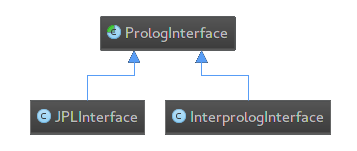
\includegraphics[width=0.8\textwidth]{img/prologInterface.png}
\end{figure}

La classe astratta conterrà i seguenti metodi:

\begin{javacode}
public abstract class PrologInterface {

  abstract void close();
  abstract void consult(File file);
  abstract void asserta(String pred, List<String> args);
  abstract void assertz(String pred, List<String> args);
  abstract void retract(String pred, List<String> args);
  abstract void retractAll(String pred, List<String> args);
  abstract boolean statisfied(String pred, List<String> args);
  abstract Map<String, String> oneSolution(String pred, List<String> args);
  abstract List<Map<String, String>> allSolutions(String pred, List<String> args);
}
\end{javacode}

\subsection{JPL Library}
\label{JPL}
\nocite{swi:jpl}
Una libreria utilizzata per permettere la bidirezionalità della comunicazione tra Java e Prolog, è stata la \emph{JPL 3.1.4 alpha}\footnote{Scaricabile da \url{http://mvnrepository.com/artifact/jpl/jpl/3.1.4-alpha}} (\textbf{J}ava-calls-\textbf{P}rolog \textbf{L}ibrary)

Le API messe a disposizione dalla libreria JPL permettono la creazione di oggetti Java che andranno a inglobare gli elementi che saranno poi utilizzati lato Prolog. La struttura gerarchica delle classi presenti nella libreria è la seguente:
\begin{Verbatim}
Term
|
+--- Variable
|
+--- Compound
|      |
|      +--- Atom
|
+--- Integer
|
+--- Float

Query

JPLException
|
+-- PrologException
\end{Verbatim}

Le classi Term-based sono in grado di adattare al meglio la concreta sintassi strutturata dei termini di Prolog, in quanto non esiste una corrispondenza diretta con un particolare termine di Prolog; piuttosto, esistono diversi significati assunti dalla classe Term, si va dalla necessità di creare delle strutture da essere utilizzate all'interno di query Prolog, fino ad arrivare al tipo di rappresentazione, con relativa esplorazione, dei risultati ottenuti dalla query.

Per astrarre quindi il concetto di termine, la classe \emph{Term} è una classe astratta istanziata da una delle sue cinque possibili sottoclassi:
\clearpage
\paragraph{Compounds}
Un Compound è un Termine che contiene un nome e una sequenza di argomenti di tipo Term.

\begin{javacode}
	Compound teacher_of = new Compound("teacher_of",
	new Term[] {
		new Atom("aristotle"),
		new Atom("alexander")
	}
	);
\end{javacode}

In questo esempio, la variabile Java \emph{teacher\_of} si riferisce a una istanza di tipo \emph{Compound} che rappresenta il termine Prolog.

\begin{prologcode}
	teacher_of(aristotle,alexander).
\end{prologcode}

\paragraph{Atom}
Un Atom è una specializzazione di \emph{Compound} avente zero parametri, il che vorrà dire che Atom sarà un Term contenente solo un nome.

\begin{javacode}
	Atom aristotle = new Atom("aristotle");
	Atom alexander = new Atom("alexander");
\end{javacode}

\paragraph{Variable}
Le Variabili sono dei Term aventi un nome identificativo il quale deve soddisfare la sintassi Prolog.

\begin{javacode}
	Variable X = new Variable("X");  //  variabile X
	Variable X = new Variable("_");  //  variabile "anonima"
	Variable X = new Variable("_Y"); // variabile Y di cui non si vuole 
	// conoscere il contenuto
\end{javacode}

\paragraph{Integer}
Un Integer è una specializzazione di \emph{Term} che mantiene la valorizzazione di tipo long di Java. Questa classe corrisponde al tipo integer di Prolog.

\begin{javacode}
	jpl.Integer i = new jpl.Integer(5);
\end{javacode}

\paragraph{Floats}
Un Float è una specializzazione di \emph{Term} che mantiene la valorizzazione di tipo double di Java. Questa classe corrisponde al tipo float di Prolog sulla quale possono essere eseguite le operazioni aritmetiche.

\begin{javacode}
	jpl.Float f = new jpl.Float(3.14159265);
\end{javacode}

\paragraph{Queries}
Ogni istanza di Query contiene un \emph{Term}, il quale rappresenta il goal da dimostrare.

\begin{javacode}
	Term goal = new Compound("teacher_of",
	  new Term[] {
		  new Atom("aristotle"),
		  new Atom("alexander")
		  }
	  );
	Query q = new Query( goal );
\end{javacode}

La query q in questo esempio rappresenta la query Prolog:

\begin{prologcode}
	?- teacher_of(aristotle,alexander).
\end{prologcode}

\subsubsection{Applicazione}
Come descritto in precedenza, nel sistema sarà presente una classe Java denominata \emph{JPLInterface} nella quale saranno implementati i diversi metodi astratti secondo le specifiche definite dalla libreria JPL; di seguito verranno mostrate le implementazioni dei principali metodi realizzati usando la libreria JPL.
\paragraph{costruttore}
Inizialmente è stato definito il costruttore della classe JPL nel quale viene settata la directory dalla quale prendere i file lib necessari a inizializzare l'oggetto JPL da creare. Definendo, in questo modo, quale interprete Prolog utilizzare tra YAP e SWI. Di seguito un estratto di codice:

\begin{javacode}
  public JPLInterface(int type) {
  
    switch (type) {
  
      case SWI:
      jpl.JPL.setNativeLibraryDir(SWI_LIB_PATH);
      
      case YAP:
      jpl.JPL.setNativeLibraryDir(YAP_LIB_PATH);
      
      default:
      break;
    }
    jpl.JPL.init();
  }
\end{javacode}

\paragraph{consult}
Nel metodo consult non si fa altro che andare a richiamare il metodo \emph{hasSolution()} di un nuovo oggetto di tipo Query avente come parametro un compound basato su un consult di un file fisico.

\begin{javacode}
  public void consult(File file) {
  	
    Term t = new Compound("consult", new Term[]{
                 new Atom(file.getAbsolutePath())
                 });
    Query query = new Query(t);
    query.hasSolution();
    query.close();
}
\end{javacode}


\paragraph{oneSolution}
Nel metodo oneSolution è stato realizzato un oggetto di tipo hashmap che dovrà contenere al suo interno il map tra i parametri passati ad un predicato Prolog e la stringa ottenuta come risultato dell'unificazione di quel predicato.
Per ottenere tali risultati si è utilizzato il metodo oneSolution della classe Query il quale restituisce l'hashtable contenente la mappatura tra stringa e Termini.
Di seguito uno stralcio di codice del metodo:

\begin{javacode}
  public Map<String, String> oneSolution(String pred, List<String> args){
  
  //Inizializzazione variabili
    Map<String, String> map = new HashMap<>();
    List<String> vars = new ArrayList<>(args.size());
    Term term;
    Term[] termArgs = new Term[args.size()];
    term = new Compound(pred, termArgs);
    
  //Creazione della query da eseguire
    Query query = new Query(term);
    
  //Esecuzione della query
    java.util.Hashtable<String, Term> ht = query.oneSolution();
    
  //Salvataggio dei risultati ottenuti
    for (String var : vars) {
      map.put(var, ht.get(var).toString());
    }
    
    return map;
\end{javacode}
\subsection{InterProlog}
\label{InterProlog}
\nocite{interprolog}
\nocite{calejo2004interprolog}
InterProlog nasce dall'esigenza di estendere in un qualche modo le potenzialità di un linguaggio dichiarativo quale è Prolog, con un secondo linguaggio, come ad esempio Java, che sia in grado di gestire le diverse problematiche che si potranno avere nello sviluppo di un sistema più ampio e complesso come la multi-piattaforma e il multi-threading.

InterProlog infatti, è un'applicazione Java open source
in grado di permettere una comunicazione bidirezionale
tra Java e Prolog attraverso il ridirezionamento dello
standard output instaurando una connessione con socket
TCP/IP tra i due linguaggi permettendo lo scambio bidirezionale
di \emph{Object} lato Java e \emph{Termini} lato Prolog, il
tutto in maniera totalmente trasparente grazie alla creazione
di API che inglobano le operazioni più a basso livello sia lato
Prolog che lato Java. In alternativa, la comunicazione può essere
realizzata attraverso l'utilizzo delle
\emph{dynamic loadable library} oppure anche usando le
interfacce native di Java.

\begin{figure}[H]
	\centering
	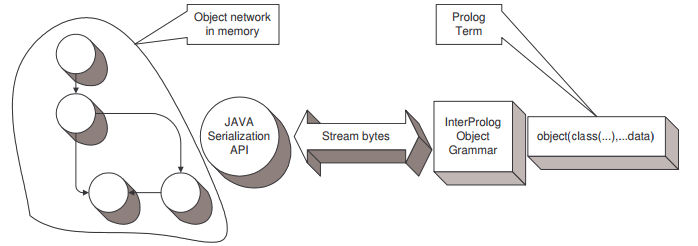
\includegraphics[width=0.9\textwidth]{img/InterPrologSystem.png}
\end{figure}

Tra le novità introdotte nelle ultime versioni di InterProlog vi è il supporto a più interpreti Prolog quali XSB, YAP, SWI:
\begin{itemize}
	\item Lato Prolog: è stato ridefinito il layer Prolog ridefinendolo in modo da essere compatibile con lo \emph{standard de facto} Prolog, inserendo parti dedicate ad ognuno dei diversi interpreti supportati.
	\item Lato Java: sono stati introdotti i diversi \emph{PrologEngine} relativi ai vari interpreti supportati.
\end{itemize}

Di seguito verrà visto il funzionamento Java-side e Prolog-side.
\subsubsection*{Java-side}
InterProlog fornisce allo sviluppatore Java delle API in grado di permettere l'accesso alla piena potenza computazionale offerta dal motore logico Prolog. Di seguito un esempio di codice usato per eseguire nell'ordine:
\begin{itemize}
	\item Inizialize: Inizializzazione del motore Prolog da usare, in questo caso l'interprete SWI;
	\item Consult: Consultazione di un file fisico tramite il comando \emph{consultAbsolute};
	\item Execute: Esecuzione del predicato \emph{descendent\_of} e salvataggio dei risultati in un array di oggetti chiamato \emph{bindings};
	\item Result: Estrazione e visualizzazione del primo risultato estratto dall'esecuzione del predicato.
\end{itemize}

\begin{javacode}
 //Init
  PrologEngine engine = new SWISubprocessEngine();
    
 //Consult
  engine.consultAbsolute("test.pl");
    
 //Execute
  Object[] bindings = engine.deterministicGoal(
                       "descendent_of( X, someAncestor )","[string(X)]");
    
 //Result
  if(bindings!=null){// succeeded
      String X = (String)bindings[0];
      System.out.println( "X = " + X);
  }
\end{javacode}

\subsubsection*{Prolog-side}
Il principale contributo offerto da InterProlog nella programmazione Prolog, è l'utilizzo del predicato \emph{javaMessage}, di seguito il codice Prolog che usa tale predicato e l'output che verrà restituito:

\begin{prologcode}
?- javaMessage('javax.swing.JFrame',W,'JFrame'(string(myTitle))),
   javaMessage(W,C,getContentPane),
   javaMessage('javax.swing.JLabel',L,
            'JLabel'(string('Hello Prolog, greetings from Swing'))),
   javaMessage(C,add(string('Center'),L)),
   javaMessage(W,pack), javaMessage(W,show).
\end{prologcode}

\begin{figure}[H]
	\centering
	
\includegraphics[width=0.4\textwidth]{img/javaMessageInterProlog.png}
\end{figure}

\subsubsection{Applicazione}
\paragraph{costruttore}
Cosi come viene fatto per la classe JPLInterface, anche in questo caso viene settato quale interprete usare tra SWI e YAP attraverso l'istanziazione dell'oggetto \emph{engine} in base al costruttore relativo all'interprete scelto.

\begin{javacode}
    private PrologEngine engine;

    public InterprologInterface(int type) {

        switch (type) {
            case SWI:
            engine = new SWISubprocessEngine(SWI_BIN_PATH, false);

            case YAP:
            engine = new YAPSubprocessEngine(YAP_BIN_PATH, false);

            default:
            break;
        }
    }
\end{javacode}
\paragraph{consult}
Il metodo consult prevede il richiamo del metodo \emph{consultAbsolute} dell'oggetto \emph{engine}, il quale permetterà di consultare il file passato come parametro al metodo.

\begin{javacode}
    public void consult(File file) {

        boolean hasSolution = engine.consultAbsolute(file);
        System.out.print("[Prolog] consult: " + file + " ");
        System.out.println(hasSolution ? "succeeded" : "failed");
    }
\end{javacode}
\paragraph{oneSolution}
Nel metodo \emph{oneSolution}, una volta inizializzate le variabili da utilizzare, creato il goal da unificare partendo dal predicato e dalla lista di argomenti che quel predicato avrà, il metodo dovrà modificare la sintassi del goal in modo tale da poter essere eseguita da InterProlog in maniera corretta; 
Ad esempio, se volessimo trovare quali siano tutte le persone taggate nel documento, il goal che si sarebbe dovuto eseguire lato Prolog sarebbe dovuto essere

\begin{prologcode}
	?- allpersona(ResultList).
\end{prologcode}

Mentre, affinché possa essere eseguito da InterProlog, il goal verrà modellato nel seguente modo:

\begin{prologcode}
	?- allpersona(ResultList), term_to_atom(ResultList, R0)
\end{prologcode}

I risultati saranno inseriti all'interno della variabile \emph{R0} di tipo stringa.
Una volta preparato il goal, si passerà all'unificazione di quest'ultimo lato Prolog attraverso l'invocazione del metodo \emph{deterministicGoal} dell'oggetto \emph{engine} definito nel costruttore.

\begin{javacode}
   public Map<String, String> oneSolution(String pred, List<String> args){
   
   //Inizializzazione variabili
     String goal = "";
     Map<String, String> map = new HashMap<>();
     List<String> vars = new ArrayList<>(args.size());

   //Creazione del goal da unificare
     goal += pred + "(";
     for (String arg : args)
       goal += arg + ",";
     goal += ")";
       
   //Creazione delle variabili da essere restituite
     String rVars = "[";
     for (int i = 0; i < vars.size(); i++) {
       goal += ", term_to_atom(" + vars.get(i) + ", R" + i + ")";
       rVars += "string(R" + i + "),";
     }
     rVars += "]";

   //Esecuzione del goal
     Object[] result = engine.deterministicGoal(goal, null, null, rVars);
     
   //Salvataggio dei risultati ottenuti
     for (int i = 0; i < result.length; i++) {
       map.put(vars.get(i), result[i].toString());
     }
      
     return map;
   }
\end{javacode}